\section{Fourth Member}

\subsection{Comments about the module}
The best part of Software Engineering, was arguably also the worst part, the lab sessions. Working in a team was fun, but could also get stressful due to the looming time constraint. Lectures were dull in all honesty, but I appreciate and realise what is required in the software engineering process, despite how depressing and long winded each of the processes may be. I'm glad we've not had to produce an IEEE SRS Document (yet?). Those standards... intimidate me. 

\subsection{Selfie with Max}

\begin{figure}[h]
\caption{Selfie with Max}
\centering
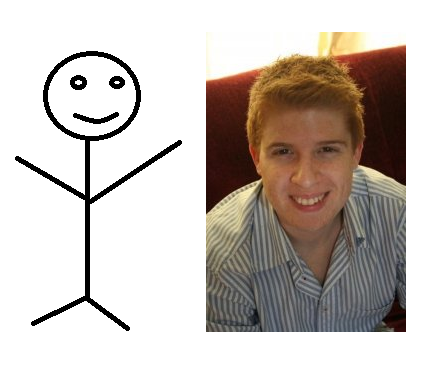
\includegraphics[width=0.5\textwidth]{superiorSelfieWithMax}
\label{fig:selfie}
\end{figure}

\subsection{What I have learned in this module}

In this module I have learnt how to engineer software. 
I have expanded my artistic skills by producing high class (literally!) diagrams.
Have you seen DAT 'SELFIE' btw? BEC DAT SELFIE. (see Figure 4 in Section 5.2)


On a serious note, the most significant aspect within this module has been working towards a deadline in a team. Due to the element of time, we realised there was a requirement for having a strategic approach towards the tasks. Not only did we have to ration out tasks during each lab session, but we would also have regular group meetings in advance during the week, to prepare and ensure we were all on the same level. This is where communication is also very important. In order to maintain consistency we would work together on single word document using Office 365, which I thought was rather useful.


Aside from all that, all the diagrams jazz, etc, etc. You know what I'm on about.

Also screw Visual Paradigm. And Office 365. And tables/images appearing in random places in all of our submitted documents.